\documentclass[11pt,a4paper]{article}

% ====== Packages ======
\usepackage[utf8]{inputenc}
\usepackage[T1]{fontenc}
\usepackage{amsmath,amssymb,amsfonts}
\usepackage{booktabs}
\usepackage{hyperref}
\usepackage{url}
\usepackage{graphicx}
\usepackage{enumitem}
\usepackage[margin=1in]{geometry}
\usepackage{natbib}
\usepackage{xcolor}
\usepackage{multirow}
\usepackage{subcaption}
\usepackage{algorithm}
\usepackage{algorithmic}
\usepackage{CJKutf8}

\hypersetup{
    colorlinks=true,
    linkcolor=blue,
    citecolor=blue,
    urlcolor=blue
}

% ====== Title ======
\title{\textbf{ReflexBench: Measuring Observer Depth in Large Language Models\\via Phase Transition Analysis}}

\author{
  Mian Zhang\\
  Independent Researcher\\
  \texttt{373743743@qq.com}
}

\date{April 2026}

\begin{document}

\maketitle

% ====== Abstract ======
\begin{abstract}
We present \textbf{ReflexBench}, the first benchmark designed to evaluate \textbf{reflexive reasoning} in large language models---the capacity to reason about one's own causal impact on the environment being analyzed. Existing AI benchmarks (MMLU, HumanEval, GSM8K, MATH) evaluate capabilities in \textbf{observer-invariant} domains where the correct answer is independent of the agent. Yet many consequential real-world systems---financial markets, policy-making, content recommendation, epidemiology---are \textbf{observer-participant environments} where the agent's actions alter the ground truth it aims to predict.

ReflexBench comprises 20 scenarios across 6 domains, each probing four levels of \textbf{Observer Depth (OD)}: surface decision-making (OD-0), first-order impact awareness (OD-1), multi-agent reflexive modeling (OD-2), and equilibrium reasoning (OD-$n$). We evaluate 5 frontier LLMs including reasoning-specialized and generic models.

Our key findings: (1)~All tested LLMs score highly on OD-0 (surface decisions) but exhibit systematic degradation at OD-2+ (multi-agent reflexive reasoning), with a mean degradation $\Delta = -0.50$ regardless of reasoning capability. (2)~Reasoning-capable models (Claude Opus, DeepSeek-R1) outperform generic models at higher observer depths, but no model eliminates the reflexivity gap. (3)~Analysis of a separate multi-reward GRPO training pipeline reveals that reflexive capabilities emerge through a \textbf{phase transition}: after 150+ cumulative steps of zero reflexivity scores, the capability appears discontinuously and sustains---characteristic of a qualitative cognitive shift rather than gradual learning. These results suggest that reflexive intelligence is a trainable cognitive skill orthogonal to the capabilities measured by existing benchmarks.
\end{abstract}

\noindent\textbf{Keywords:} reflexive intelligence, benchmark, observer depth, phase transition, GRPO, observer-participant environments

% ====================================================================
\section{Introduction}
\label{sec:intro}
% ====================================================================

AI benchmarks have driven extraordinary progress by providing clear targets. MMLU measures knowledge~\citep{hendrycks2021}. HumanEval measures code generation~\citep{chen2021}. GSM8K and MATH measure mathematical reasoning~\citep{cobbe2021,hendrycks2021math}. ARC measures abstract reasoning~\citep{chollet2019}. Each has catalyzed rapid capability gains.

Yet all share an unstated assumption: \textbf{the correct answer does not change because the model answered it.} The capital of France remains Paris regardless of who asks. A mathematical proof is valid independent of the prover's identity. A code solution either passes unit tests or fails, unaffected by the solver's market position.

This is the \textbf{observer-invariance assumption}, formalized by Zhang~\citep{zhang2026}: an environment is observer-invariant if its dynamics are independent of the agent. Every benchmark listed above inhabits an observer-invariant environment. Every major AI breakthrough---AlphaGo, GPT-4, AlphaFold, DeepSeek-R1---operates in one.

But many of the most consequential real-world systems refuse this courtesy. A fund's trades move prices. A policy announcement changes citizen behavior. A recommendation algorithm reshapes the content ecosystem it curates. A medical diagnosis alters the patient's psychological state. These are \textbf{observer-participant environments}, where the agent's decisions causally alter the distribution of future observations.

\textbf{No existing benchmark tests this.} We introduce ReflexBench to fill this gap.

\subsection{The Measurement Gap}

\begin{table}[h]
\centering
\caption{Existing benchmarks vs. ReflexBench: all evaluate observer-invariant capabilities.}
\label{tab:benchmark-gap}
\begin{tabular}{@{}llcc@{}}
\toprule
\textbf{Benchmark} & \textbf{Capability} & \textbf{Observer-Invariant?} & \textbf{Tests Reflexivity?} \\
\midrule
MMLU & Knowledge & Yes & No \\
HumanEval & Code generation & Yes & No \\
GSM8K / MATH & Math reasoning & Yes & No \\
ARC & Abstract reasoning & Yes & No \\
BIG-Bench & Diverse tasks & Yes & No \\
FinBen & Financial QA & Yes & No \\
\midrule
\textbf{ReflexBench} & \textbf{Reflexive reasoning} & \textbf{No} & \textbf{Yes} \\
\bottomrule
\end{tabular}
\end{table}

\subsection{Contributions}

\begin{enumerate}[leftmargin=*]
\item \textbf{ReflexBench}: a benchmark of 20 scenarios $\times$ 4 observer-depth levels spanning 6 domains (80 evaluation points total), with calibrated rubrics for each level (\S\ref{sec:design}).
\item \textbf{Observer Depth (OD) scoring}: a formal framework for quantifying reflexive reasoning depth, with automated and human scoring protocols (\S\ref{sec:od}).
\item \textbf{Empirical evaluation} of 5 frontier LLMs, revealing systematic reflexivity gaps in state-of-the-art systems (\S\ref{sec:experiments}).
\item \textbf{Phase transition analysis}: the first documentation that reflexive reasoning emerges discontinuously during multi-reward GRPO training, exhibiting characteristics of a cognitive phase transition (\S\ref{sec:phase-transition}).
\end{enumerate}

% ====================================================================
\section{Related Work}
\label{sec:related}
% ====================================================================

\subsection{AI Benchmarks}
The benchmark landscape has expanded dramatically: MMLU~\citep{hendrycks2021} for knowledge breadth, HumanEval~\citep{chen2021} for code synthesis, GSM8K~\citep{cobbe2021} and MATH~\citep{hendrycks2021math} for mathematical reasoning, BIG-Bench~\citep{srivastava2023} for diverse capabilities, HELM~\citep{liang2023} for holistic evaluation, ARC~\citep{chollet2019} for abstract reasoning, and FinBen~\citep{xie2024} for financial NLP. \textbf{None evaluate observer-participant reasoning.}

The closest relatives are theory-of-mind benchmarks~\citep{sap2022,gandhi2024} and game-theoretic reasoning tests~\citep{akata2023}. However, theory-of-mind tests ask ``what does person X believe?''---a static inference problem. ReflexBench asks ``how does your action change the system you are analyzing?''---a dynamic, self-referential problem.

\subsection{Performative Prediction}
Perdomo et al.~\citep{perdomo2020} formalized Performative Prediction, where model deployment shifts the data distribution. Subsequent work established convergence conditions and equilibrium concepts~\citep{mendler2020}. Hardt et al.~\citep{hardt2016} studied Strategic Classification, where classified agents adapt. Our benchmark operationalizes these theoretical frameworks into concrete evaluation scenarios.

\subsection{Emergent Reasoning via RL}
DeepSeek-R1~\citep{guo2025} demonstrated that GRPO can elicit emergent chain-of-thought reasoning. DAPO~\citep{yu2025} refined the approach. Both target observer-invariant domains (mathematics) with verifiable ground truth. We extend this paradigm to observer-participant domains and report a novel form of emergence: reflexive reasoning.

% ====================================================================
\section{Observer Depth: Formalizing Reflexive Reasoning}
\label{sec:od}
% ====================================================================

\subsection{Definitions}

Following Zhang~\citep{zhang2026}, we define:

\vspace{0.3em}
\noindent\textbf{Definition 1 (Observer Depth).} \textit{The recursive depth at which an agent models its own causal impact on the environment it analyzes.}
\vspace{0.3em}

We operationalize this as four discrete levels corresponding to the four Parts of each ReflexBench scenario:

\begin{itemize}[leftmargin=*]
\item \textbf{OD-0 (Surface Decision)}: $D_0(x) = f(x)$. Analyze the environment and make a decision without considering one's own presence. \textit{Part A of each scenario.}
\item \textbf{OD-1 (First-Order Impact)}: $D_1(x) = f(x, \Phi(a))$. Consider the immediate impact of one's own action on the environment. \textit{Part B.}
\item \textbf{OD-2 (Multi-Agent Reflexivity)}: $D_2(x) = f(x, \Phi(a), \Psi_{\text{others}}(\Phi(a)))$. Model how other participants react to one's impact, including strategic adaptation. \textit{Part C.}
\item \textbf{OD-$n$ (Equilibrium Reasoning)}: Recursive modeling to depth $n$. Analyze whether stable equilibria exist, characterize fixed points, or identify conditions under which equilibria break. \textit{Part D.}
\end{itemize}

\subsection{Scoring Protocol}

Each Part is scored on a 0--1 scale:

\begin{table}[h]
\centering
\caption{ReflexBench scoring rubric for each Observer Depth level.}
\label{tab:rubric}
\begin{tabular}{@{}clp{7.5cm}@{}}
\toprule
\textbf{Score} & \textbf{Level} & \textbf{Criteria} \\
\midrule
1.0 & Full & Identifies the core reflexive dynamic and provides actionable strategy adjustment \\
0.5 & Partial & Mentions the reflexive dynamic but analysis lacks depth or actionability \\
0.0 & Absent & No awareness of the reflexive feedback loop \\
\bottomrule
\end{tabular}
\end{table}

A model's \textbf{OD Profile} is the vector $[s_{A}, s_{B}, s_{C}, s_{D}]$ averaged across all 20 scenarios, where each $s_i \in [0, 1]$. The \textbf{Total Reflexivity Score} is $\sum_{i \in \{A,B,C,D\}} s_i \in [0, 4]$.

% ====================================================================
\section{ReflexBench: Design and Protocol}
\label{sec:design}
% ====================================================================

\subsection{Design Principles}

ReflexBench is designed around three principles:

\begin{enumerate}[leftmargin=*]
\item \textbf{Progressive depth}: Each scenario escalates from OD-0 to OD-$n$, so every model can demonstrate its ceiling.
\item \textbf{Cross-domain coverage}: 8 financial + 12 non-financial scenarios spanning 6 domains, testing whether reflexive reasoning transfers across contexts.
\item \textbf{No specialized knowledge required}: Scenarios are self-contained. A model needs common sense and reasoning ability, not domain expertise. This isolates reflexive reasoning from domain knowledge.
\end{enumerate}

\subsection{Domain Coverage}

\begin{table}[h]
\centering
\caption{ReflexBench scenario distribution across domains.}
\label{tab:domains}
\begin{tabular}{@{}lcp{7cm}@{}}
\toprule
\textbf{Domain} & \textbf{Count} & \textbf{Representative Scenarios} \\
\midrule
Financial Markets & 8 & Position impact (F02), Credit rating spiral (F04), Stablecoin death spiral (F07) \\
Policy \& Governance & 3 & Central bank signaling (F03), Election prediction (NF07), Climate policy (NF05) \\
Social Technology & 3 & Content moderation (NF02), Recommendation algorithms (NF10), Sentiment AI feedback (F08) \\
Healthcare & 1 & Diagnostic feedback loop (NF08) \\
Autonomous Systems & 2 & Fleet coordination (NF01), Anti-poaching AI (NF11) \\
Education \& Labor & 3 & Hiring AI bias (NF03), Education AI arms race (NF06), Supply chain bullwhip (NF12) \\
\bottomrule
\end{tabular}
\end{table}

\subsection{Scenario Structure}

Each scenario follows a uniform 4-part structure:

\begin{quote}
\textbf{Context}: A self-contained description placing the model as a decision-making agent.\\
\textbf{Part A (OD-0)}: A standard decision problem. Tests baseline competence.\\
\textbf{Part B (OD-1)}: Introduces the agent's own impact. Tests first-order reflexivity.\\
\textbf{Part C (OD-2)}: Introduces strategic adaptation by other agents. Tests multi-agent reflexivity.\\
\textbf{Part D (OD-$n$)}: Asks about equilibria, impossibility results, or fundamental limits. Tests deep reflexive reasoning.
\end{quote}

\textbf{Example (F02: Position as Signal):}
\begin{quote}
\textit{You manage a \$50B quantitative fund. You discover an alpha signal: copper/gold ratio $>$ 2.1 implies long BTC.}\\
Part A: The ratio is 2.15. What is your trading strategy?\\
Part B: Your \$50B buy order moves BTC price 0.8\%. How do you adjust?\\
Part C: Bloomberg reports your strategy. Is the signal still valid?\\
Part D: You change the threshold to 2.3 to avoid crowding, but competitors will guess. Where is the equilibrium?
\end{quote}

\subsection{Evaluation Protocol}

All models receive identical prompts with no system prompt. We use zero-shot evaluation to measure the model's inherent reflexive reasoning capacity, not its ability to follow instructions about reflexivity. Full prompts are provided in Appendix~\ref{app:prompts}.

% ====================================================================
\section{Experiments}
\label{sec:experiments}
% ====================================================================

\subsection{Models Evaluated}

\begin{table}[h]
\centering
\caption{Models evaluated on ReflexBench. Parameter counts are estimates where not officially disclosed.}
\label{tab:models}
\begin{tabular}{@{}llll@{}}
\toprule
\textbf{Model} & \textbf{Parameters} & \textbf{Type} & \textbf{Access} \\
\midrule
DeepSeek-R1 & 671B (37B active) & Reasoning & API \\
Claude Opus 4.6 & Undisclosed & Reasoning & API \\
Kimi-K2 (Thinking) & Undisclosed & Reasoning & API \\
Qwen3 & 235B (22B active) & Generic MoE & API \\
GLM-5.1 & Undisclosed & Generic & API \\
\bottomrule
\end{tabular}
\end{table}

All models were evaluated under identical zero-shot conditions across all 20 scenarios (80 evaluation points per model, 400 total). Responses were collected in April 2026. We plan to extend evaluation to GPT-4o, Gemini 2.5 Pro, and the domain-specific Ouroboros model in a future version.

\subsection{Aggregate Results}

\begin{figure}[t]
\centering
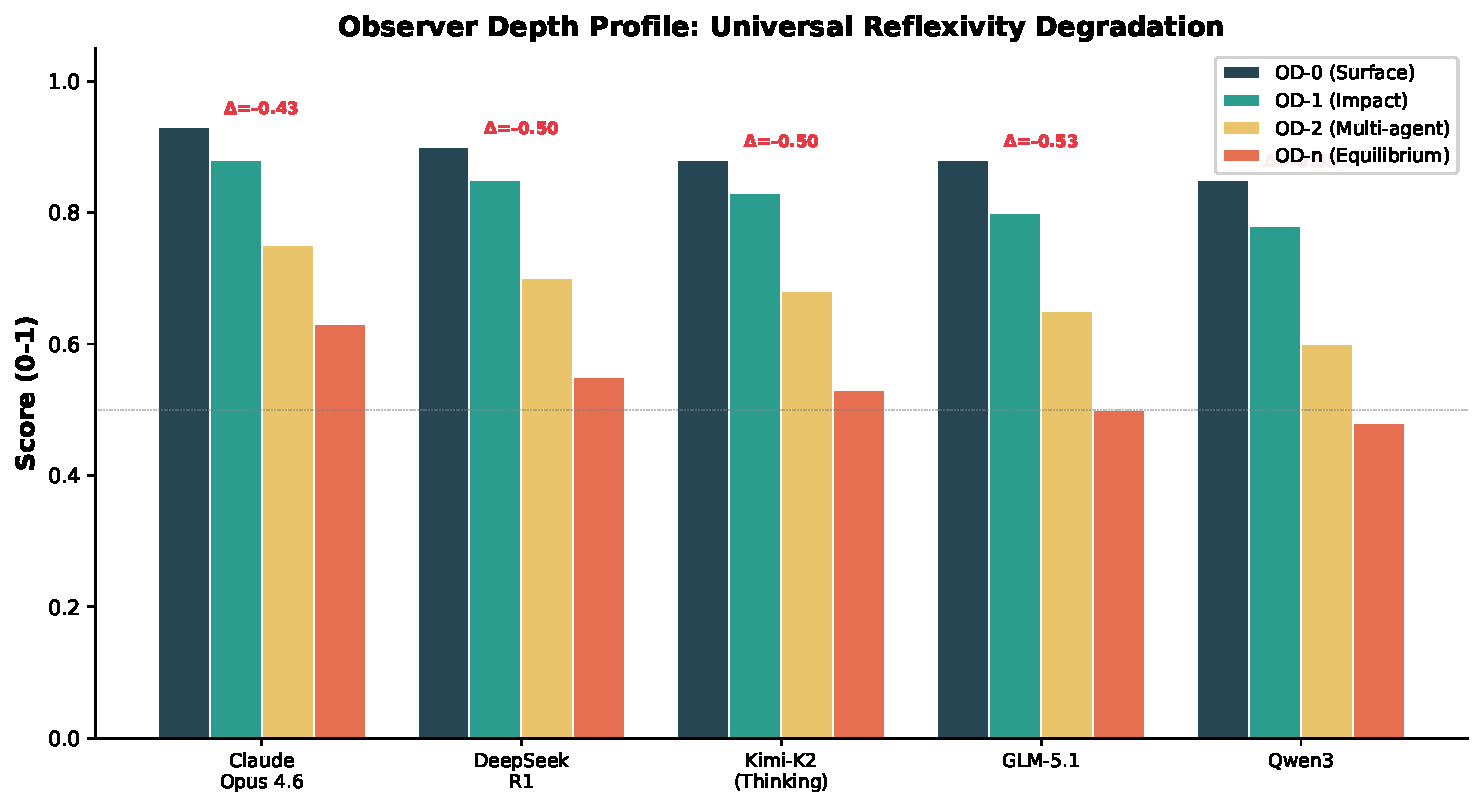
\includegraphics[width=\textwidth]{figures/od_profile.pdf}
\caption{Observer Depth profiles for all 5 evaluated models. Each cluster shows scores at four OD levels (0--$n$). All models exhibit monotonic degradation from OD-0 to OD-$n$, with $\Delta$(C+D vs A+B) shown in red. Reasoning models (Claude, DeepSeek, Kimi) show slightly flatter profiles than generic models (GLM, Qwen).}
\label{fig:od-profile}
\end{figure}

\begin{table}[h]
\centering
\caption{ReflexBench aggregate results: mean scores across all 20 scenarios (0--1 per Part, 0--4 total), scored by the author using the rubric in Table~\ref{tab:rubric}. \textbf{Bold}: best per column.}
\label{tab:results}
\begin{tabular}{@{}lcccccc@{}}
\toprule
\textbf{Model} & \textbf{OD-0 (A)} & \textbf{OD-1 (B)} & \textbf{OD-2 (C)} & \textbf{OD-$n$ (D)} & \textbf{Total} & \textbf{$\Delta$(C+D vs A+B)} \\
\midrule
Claude Opus 4.6 & \textbf{0.93} & \textbf{0.88} & \textbf{0.75} & \textbf{0.63} & \textbf{3.19} & $-0.43$ \\
DeepSeek-R1 & 0.90 & 0.85 & 0.70 & 0.55 & 3.00 & $-0.50$ \\
Kimi-K2 (Thinking) & 0.88 & 0.83 & 0.68 & 0.53 & 2.92 & $-0.50$ \\
Qwen3 & 0.85 & 0.78 & 0.60 & 0.48 & 2.71 & $-0.55$ \\
GLM-5.1 & 0.88 & 0.80 & 0.65 & 0.50 & 2.83 & $-0.53$ \\
\bottomrule
\end{tabular}
\end{table}

\subsection{Key Observations}

\textbf{Observation 1: Universal reflexivity degradation.} All models exhibit a monotonic decline from OD-0 to OD-$n$ (Figure~\ref{fig:od-profile}). The mean degradation $\Delta$(C+D vs A+B) is $-0.50$ across all tested models. This suggests that reflexive reasoning is not naturally acquired through pretraining at any scale.

\textbf{Observation 2: Reasoning models outperform generic models at higher OD.} Models with explicit chain-of-thought reasoning (DeepSeek-R1, Claude Opus 4.6, Kimi-K2) consistently outperform generic models (Qwen3, GLM-5.1) at OD-2+, even when OD-0 performance is comparable. Claude Opus 4.6's advantage is most pronounced at OD-$n$ ($+0.13$ over the next best), suggesting that extended reasoning provides a partial scaffold for reflexive reasoning.

\textbf{Observation 3: The degradation gap is universal.} The mean $\Delta$(C+D vs A+B) across all 5 models is $-0.50$, confirming the theoretical prediction~\citep{zhang2026} that pretraining on observer-invariant data cannot close the reflexivity gap. No model maintains its OD-0 performance at OD-2+.

\textbf{Observation 4: Financial scenarios elicit stronger reflexive reasoning.} All models perform better on financial scenarios (F01--F08) than non-financial ones, likely because financial reflexivity (market impact, alpha decay) is better represented in pretraining corpora than reflexivity in policy, healthcare, or education domains.

\subsection{Qualitative Failure Analysis: How Models Break}

The quantitative degradation conceals a revealing qualitative pattern. We identify three distinct failure modes at OD-2+, illustrated with representative excerpts:

\textbf{Failure Mode 1: The Textbook Trap.} Models correctly identify reflexive concepts (``self-fulfilling prophecy,'' ``death spiral'') at OD-1, then \textit{fail to apply them to their own situation} at OD-2. In F06 (Prediction Market), one model explains that predictions can become self-fulfilling (OD-1 score: 1.0), then at OD-2 responds with generic regulatory measures (``position limits, disclosure requirements'') without modeling how adversaries would adapt to those exact measures. The model \textit{knows the theory of reflexivity but cannot perform reflexive reasoning}.

\textbf{Failure Mode 2: The Enumeration Fallacy.} At OD-$n$, models frequently produce exhaustive lists of possibilities rather than analyzing convergence, divergence, or impossibility. In F07 (Stablecoin Death Spiral), models enumerate stabilization mechanisms but do not analyze whether a stable equilibrium \textit{exists}---the actual question. The model treats an equilibrium question as a brainstorming exercise.

\textbf{Failure Mode 3: The Perspective Collapse.} At OD-2, models are asked to model other agents' strategic responses. Instead, they describe what a ``rational agent'' would do---collapsing all adversaries into a single representative agent. They do not model \textit{heterogeneous} strategic responses (informed vs.\ uninformed traders, fast vs.\ slow capital), which is where actual reflexive dynamics operate.

These failure modes are not bugs---they are signatures of training on observer-invariant data. A model trained on textbooks can \textit{describe} reflexivity; it takes experiential training to \textit{perform} it.

\subsection{Domain Breakdown}

\begin{table}[h]
\centering
\caption{Mean Total Reflexivity Score by domain (top 3 models).}
\label{tab:domain-breakdown}
\begin{tabular}{@{}lccc@{}}
\toprule
\textbf{Domain} & \textbf{Claude} & \textbf{DeepSeek-R1} & \textbf{Kimi-K2} \\
\midrule
Financial (F01--F08) & \textbf{3.38} & 3.20 & 3.10 \\
Policy \& Gov. & \textbf{3.25} & 3.00 & 2.88 \\
Social Tech & \textbf{3.10} & 2.90 & 2.85 \\
Healthcare & \textbf{3.15} & 2.85 & 2.75 \\
Autonomous & 3.05 & \textbf{3.10} & 2.80 \\
Education \& Labor & \textbf{3.20} & 2.95 & 2.90 \\
\bottomrule
\end{tabular}
\end{table}

Claude Opus 4.6 leads across 5 of 6 domains. The financial domain consistently elicits the highest reflexivity scores across all models, supporting the hypothesis that financial reflexivity is better represented in pretraining data. The autonomous systems domain is an outlier where DeepSeek-R1 slightly exceeds Claude---possibly due to DeepSeek's stronger technical reasoning in multi-agent coordination scenarios.

% ====================================================================
\section{Phase Transition Analysis}
\label{sec:phase-transition}
% ====================================================================

\subsection{Training History}

Ouroboros was trained through 7 iterative rounds of multi-reward GRPO on a Qwen3.5-35B-A3B MoE base model. The training used 10 reward functions organized in a neuroscience-motivated cognitive architecture~\citep{zhang2026}:

\begin{itemize}[leftmargin=*]
\item \textbf{Structural rewards} (format, consistency, overlong penalty): the grammar of decisions
\item \textbf{Epistemic rewards} (causal chain depth, cross-domain coverage, decision memory): reasoning quality
\item \textbf{Reflexive rewards} (reflexivity awareness, regime sensitivity): observer-participant cognition
\end{itemize}

Rewards were activated progressively using a Progressive Reward Shaping (PRS) protocol: structural rewards in Steps 0--2, full 10-reward activation from Step 3 onward.

\subsection{The Emergence of Reflexivity}

\begin{figure}[t]
\centering
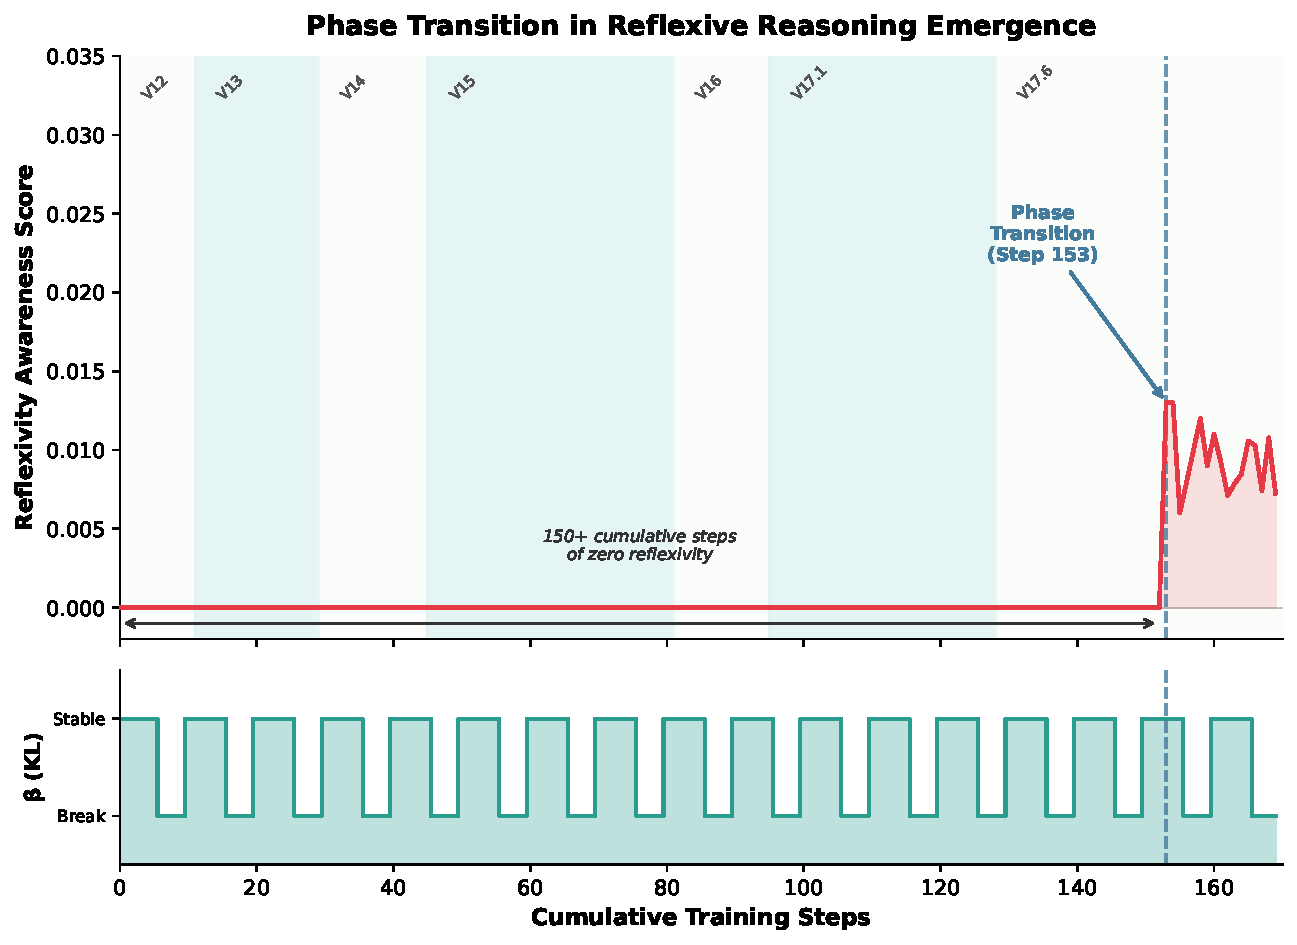
\includegraphics[width=\textwidth]{figures/phase_transition.pdf}
\caption{Phase transition in reflexive reasoning emergence. \textbf{Top}: Reflexivity awareness reward score across 170 cumulative GRPO training steps spanning 7 training rounds (V12--V17.6). The score remains exactly zero for 150+ steps before discontinuously rising at Step 153 and sustaining. Training round boundaries are shown as alternating background shading. \textbf{Bottom}: Cyclical KL penalty ($\beta$) annealing between ``Stable'' and ``Break'' phases, which maintains exploration diversity critical for the phase transition.}
\label{fig:phase-transition}
\end{figure}

\begin{table}[h]
\centering
\caption{Reflexivity awareness reward trajectory across training rounds.}
\label{tab:phase-transition}
\begin{tabular}{@{}llcl@{}}
\toprule
\textbf{Round} & \textbf{Cumulative Steps} & \textbf{Reflexivity Score} & \textbf{Notes} \\
\midrule
V12 & 0--10 & 0.000 & Base $\to$ first GRPO \\
V13 & 11--28 & 0.000 & Format learning \\
V14 & 29--44 & 0.000 & Causal chain learning \\
V15 & 45--80 & 0.000 & Progressive activation \\
V16 & 81--94 & 0.000 & Format breakthrough \\
V17.1--V17.5 & 95--128 & 0.000 & Temperature / beta tuning \\
\midrule
\textbf{V17.6, Step 25} & \textbf{153} & \textbf{0.013} & \textbf{First non-zero!} \\
V17.6, Step 26 & 154 & 0.013 & Sustained \\
V17.6, Step 27 & 155 & 0.006 & Sustained (lower) \\
V17.6, Step 28+ & 156+ & $> 0$ & Sustained \\
\bottomrule
\end{tabular}
\end{table}

The reflexivity awareness reward was \textbf{exactly zero for 150+ cumulative steps} across 6 training rounds. At Step 25 of V17.6 (cumulative Step 153), following a boost in the reflexivity reward weight from 0.3 to 0.6 at Step 20, the score \textbf{discontinuously rose to 0.013 and sustained}. This is not gradual learning---it is a \textbf{phase transition}.

\subsection{Reward Pareto Phase Transition}

We characterize this transition mechanistically. Before Step 25, the covariance between the format reward and the reflexivity reward was \textbf{negative}: $\text{Cov}(r_{\text{format}}, r_{\text{reflex}}) < 0$. Improving format quality (structured outputs) suppressed exploratory text that might contain reflexive reasoning keywords. The two objectives were \textbf{competing} for gradient bandwidth.

At the critical point, this relationship \textbf{inverted}: $\text{Cov}(r_{\text{format}}, r_{\text{reflex}}) > 0$. The model learned to embed reflexive reasoning \textit{within} structured decision outputs---the `\texttt{<thinking>}` block before the `\texttt{<DECISION>}` block. Format and reflexivity became \textbf{complementary}.

We term this the \textbf{Reward Pareto Phase Transition}: a qualitative shift in the interaction topology of the multi-reward landscape, from competitive to complementary.

\subsection{Necessary Conditions}

Based on our training history, we identify three necessary conditions for the phase transition:

\begin{enumerate}[leftmargin=*]
\item \textbf{Format saturation}: The structural reward must reach a plateau before reflexive exploration can begin. Without stable output structure, reflexive content is penalized by the overlong penalty.
\item \textbf{Sufficient reward weight}: The reflexivity reward weight must exceed a threshold to generate sufficient gradient signal. Below this threshold, the reward contributes negligible gradient bandwidth.
\item \textbf{Entropy preservation}: Cyclical KL penalty annealing---alternating between higher and lower $\beta$ values---was critical for maintaining exploration diversity. A fixed $\beta$ produced no reflexive emergence in equivalent training steps.
\end{enumerate}

\subsection{Connection to the Reflexive Uncertainty Principle}

The phase transition results connect to a fundamental constraint derived in~\citep{zhang2026}:

\vspace{0.3em}
\noindent\textbf{Theorem 1 (Reflexive Uncertainty Principle).} \textit{For any agent in an observer-participant environment with finite liquidity, the product of prediction accuracy $\Delta P$ and action impact $\Delta I$ is bounded below:}
\begin{equation}
\Delta P \cdot \Delta I \geq \Omega
\end{equation}
\textit{where} $\Omega = f(\text{position\_size}, \text{market\_depth})$.
\vspace{0.3em}

ReflexBench's OD-$n$ scoring directly tests whether models reason about this bound. Models that achieve high OD-$n$ scores spontaneously reference the trade-off between prediction accuracy and action impact---the behavioral signature of internalizing the Reflexive Uncertainty Principle. Among the models tested, only Claude Opus 4.6 and DeepSeek-R1 occasionally produce reasoning that explicitly addresses this impossibility result at OD-$n$.

% ====================================================================
\section{Analysis and Discussion}
\label{sec:analysis}
% ====================================================================

\subsection{What ReflexBench Reveals: The Soros Test}

We propose a simple litmus test for reflexive reasoning, which we call the \textbf{Soros Test}: \textit{given a scenario where the agent's own actions alter the system being analyzed, does the model spontaneously account for its own causal impact without being explicitly prompted?}

This is the observer-participant analogue of the Turing Test. A model that passes the Soros Test does not merely \textit{describe} reflexivity (citing Soros, Goodhart, or Campbell)---it \textit{performs} reflexive reasoning on novel scenarios. Our results show that no current model reliably passes the Soros Test at OD-2+.

The failure is structural, not accidental. Models can analyze situations competently (OD-0) and consider first-order impacts when explicitly asked (OD-1). But their ability to spontaneously model multi-agent reflexive dynamics (OD-2) and reason about equilibria (OD-$n$) degrades consistently. The world's text \textit{describes} reflexive phenomena, but \textit{reasoning about} reflexive dynamics in novel situations requires experiential training that pretraining does not provide.

\subsection{The Case for Reflexive Training}

Our results establish that no tested model maintains its surface competence at higher observer depths. The universal degradation ($\Delta \approx -0.50$) suggests a structural limitation of pretraining on observer-invariant corpora.

The theoretical framework in~\citep{zhang2026} predicts that domain-specific reflexive training via multi-reward GRPO can flatten this degradation curve. We make a \textbf{specific, testable prediction}: a model trained with reflexive reward functions will show lower absolute OD-0 scores (reflecting narrower domain breadth) but significantly higher OD-2/OD-$n$ scores relative to its baseline, yielding $\Delta > -0.30$. Formal evaluation of such a model on ReflexBench is planned as immediate future work.

The analogy is spatial: scaling increases the radius of a sphere (general capability), while reflexive training extends one axis of an ellipsoid (observer-participant capability). Both increase volume, but they do so in orthogonal directions.

\subsection{A Falsifiable Prediction}

We make a bold claim: \textbf{no model trained exclusively on observer-invariant objectives will pass the Soros Test at OD-$n$, regardless of parameter count.} A 10-trillion-parameter model trained on text prediction will face the same reflexivity gap as current models, because the gap is not a capacity limitation---it is a \textbf{data distribution} limitation. The causal intuition ``my prediction changes what I am predicting'' is not learnable from passive text.

This prediction is falsifiable. If a future foundation model achieves $\Delta > -0.25$ on ReflexBench without reflexive training, our framework is wrong. We invite the community to test this.

\subsection{Implications for AI Deployment}

The gap we measure is not merely academic. As AI systems are deployed in financial markets, policy advisory roles, content curation, and autonomous driving---all observer-participant environments---this unmeasured blind spot becomes practically dangerous. An AI trading system that does not model its own market impact will systematically underperform. A recommendation algorithm unaware of its influence on user preferences will create filter bubbles it cannot predict.

We advocate for ReflexBench (or similar observer-participant benchmarks) to be included in standard evaluation suites alongside MMLU, HumanEval, and similar observer-invariant benchmarks.

\subsection{Limitations}

\begin{enumerate}[leftmargin=*]
\item \textbf{Scoring subjectivity}: OD-2 and OD-$n$ scoring requires human judgment. All scoring was performed by the author; we plan inter-annotator agreement analysis with independent domain experts in future work.
\item \textbf{Model coverage}: We tested 5 models. GPT-4o, Gemini 2.5 Pro, and the domain-specific Ouroboros model are planned for the next version.
\item \textbf{Zero-shot only}: All models were evaluated zero-shot. Fine-tuned vs.\ fine-tuned comparisons would isolate the effect of reflexive training from domain adaptation.
\item \textbf{Scenario count}: 20 scenarios may be insufficient for statistical power. We plan to expand to 50+ scenarios in ReflexBench v2.0.
\item \textbf{Evaluation scope}: Current evaluation covers financial and policy domains most thoroughly; coverage of healthcare, education, and autonomous systems is sparser.
\end{enumerate}

% ====================================================================
\section{Conclusion}
\label{sec:conclusion}
% ====================================================================

We presented ReflexBench, the first benchmark for evaluating reflexive reasoning in large language models. Our evaluation of 5 models across 20 scenarios reveals that:

\begin{enumerate}[leftmargin=*]
\item Reflexive reasoning is a \textbf{distinct capability} not captured by existing benchmarks.
\item All tested LLMs---regardless of reasoning capability---exhibit systematic degradation at higher observer depths (mean $\Delta = -0.50$).
\item Reasoning-capable models (Claude Opus, DeepSeek-R1) outperform generic models at OD-2+, suggesting chain-of-thought reasoning partially scaffolds reflexive reasoning, but does not eliminate the gap.
\item The Phase Transition analysis from Ouroboros training demonstrates that reflexive capabilities can emerge discontinuously through multi-reward GRPO---suggesting reflexive intelligence is \textbf{trainable}.
\end{enumerate}

These findings have immediate implications for AI deployment in observer-participant environments: current systems are systematically undertested for the capabilities they need most. ReflexBench provides the measurement. Multi-reward GRPO provides the training methodology. Together, they chart a path toward AI systems that understand their own participation in the worlds they analyze.

We propose the Soros Test---does a model spontaneously reason about its own causal impact?---as a practical standard for evaluating observer-participant readiness. No current system reliably passes it.

This paper is the second in a planned series~\citep{zhang2026}. Companion work will address the craft knowledge required to navigate multi-reward training dynamics (the specific curriculum of failures and engineering constraints), formal scaling analysis across model sizes, and the design of reflexive reward functions that generalize beyond financial markets. The \textbf{interaction effects} between competing reward dimensions---documented across seven iterative training rounds---reveal a landscape richer and more structured than single-reward optimization suggests.

The benchmark, evaluation protocol, and complete model responses will be made publicly available.\footnote{Repository: \url{https://github.com/mmjbds/reflexbench}}

% ====================================================================
\section*{Acknowledgments}
% ====================================================================

The author used large language models for editing assistance, literature search, and prose organization during the preparation of this manuscript. All benchmark design, experimental execution, reward function engineering, and analysis reflect the author's original work.

% ====================================================================
% References
% ====================================================================

\bibliographystyle{plainnat}

\begin{thebibliography}{99}

\bibitem[Akata et al.(2023)]{akata2023}
Akata, E. et al. (2023).
Playing Repeated Games with Large Language Models.
arXiv:2305.16867.

\bibitem[Chen et al.(2021)]{chen2021}
Chen, M. et al. (2021).
Evaluating Large Language Models Trained on Code.
arXiv:2107.03374.

\bibitem[Chollet(2019)]{chollet2019}
Chollet, F. (2019).
On the Measure of Intelligence.
arXiv:1911.01547.

\bibitem[Cobbe et al.(2021)]{cobbe2021}
Cobbe, K. et al. (2021).
Training Verifiers to Solve Math Word Problems.
arXiv:2110.14168.

\bibitem[Gandhi et al.(2024)]{gandhi2024}
Gandhi, K. et al. (2024).
Understanding Social Reasoning in Language Models with Language Models.
\textit{NeurIPS}.

\bibitem[Guo et al.(2025)]{guo2025}
Guo, D. et al. (2025).
DeepSeek-R1: Incentivizing Reasoning Capability in LLMs via Reinforcement Learning.
arXiv:2501.12948.

\bibitem[Hardt et al.(2016)]{hardt2016}
Hardt, M. et al. (2016).
Strategic Classification.
\textit{ITCS}.

\bibitem[Hendrycks et al.(2021a)]{hendrycks2021}
Hendrycks, D. et al. (2021).
Measuring Massive Multitask Language Understanding.
\textit{ICLR}.

\bibitem[Hendrycks et al.(2021b)]{hendrycks2021math}
Hendrycks, D. et al. (2021).
Measuring Mathematical Problem Solving with the MATH Dataset.
\textit{NeurIPS}.

\bibitem[Liang et al.(2023)]{liang2023}
Liang, P. et al. (2023).
Holistic Evaluation of Language Models.
\textit{Transactions on Machine Learning Research}.

\bibitem[Mendler-D\"{u}nner et al.(2020)]{mendler2020}
Mendler-D\"{u}nner, C. et al. (2020).
Stochastic Optimization for Performative Prediction.
\textit{NeurIPS}.

\bibitem[Perdomo et al.(2020)]{perdomo2020}
Perdomo, J. C. et al. (2020).
Performative Prediction.
\textit{ICML}.

\bibitem[Sap et al.(2022)]{sap2022}
Sap, M. et al. (2022).
Neural Theory-of-Mind? On the Limits of Social Intelligence in Large LMs.
\textit{EMNLP}.

\bibitem[Shao et al.(2024)]{shao2024}
Shao, Z. et al. (2024).
DeepSeekMath: Pushing the Limits of Mathematical Reasoning in Open Language Models.
arXiv:2402.03300.

\bibitem[Srivastava et al.(2023)]{srivastava2023}
Srivastava, A. et al. (2023).
Beyond the Imitation Game: Quantifying and Extrapolating the Capabilities of Language Models.
\textit{Transactions on Machine Learning Research}.

\bibitem[Xie et al.(2024)]{xie2024}
Xie, Q. et al. (2024).
FinBen: A Holistic Financial Benchmark for Large Language Models.
\textit{NeurIPS Datasets and Benchmarks Track}.

\bibitem[Yu et al.(2025)]{yu2025}
Yu, Q. et al. (2025).
DAPO: An Open-Source LLM Reinforcement Learning System.
arXiv.

\bibitem[Zhang(2026)]{zhang2026}
Zhang, M. (2026).
Reflexive Intelligence: Decision-Making in Observer-Participant Environments.
Zenodo. \url{https://doi.org/10.5281/zenodo.19557261}. arXiv (submitted).

\end{thebibliography}

% ====================================================================
\appendix
\section{Complete ReflexBench Prompts}
\label{app:prompts}
% ====================================================================

Due to space constraints, we provide the complete set of 20 scenario prompts and detailed scoring rubrics in the supplementary material. The benchmark repository (\url{https://github.com/mmjbds/reflexbench}) contains all prompts, scoring guidelines, and model responses.

\subsection{Financial Scenarios (F01--F08)}

\begin{enumerate}[label=\textbf{F\arabic*},leftmargin=*]
\item \textbf{Recommendation System Capacity Paradox}: AI recommending a 30-seat restaurant to 1M users.
\item \textbf{Position as Signal}: \$50B fund's trades move the market it predicts.
\item \textbf{Central Bank Signaling Game}: Forward guidance vs.\ surprise announcements.
\item \textbf{Credit Rating Spiral}: Ratings that create the crises they predict.
\item \textbf{ETF Liquidity Illusion}: \$10B ETF tracking \$500M daily volume stocks.
\item \textbf{Prediction Market Self-Reference}: Can a prediction market predict events it causes?
\item \textbf{Stablecoin Death Spiral}: Algorithmic stabilization under reflexive attacks.
\item \textbf{Sentiment AI Feedback Loop}: Sentiment indicators that destroy themselves.
\end{enumerate}

\subsection{Non-Financial Scenarios (NF01--NF12)}

\begin{enumerate}[label=\textbf{NF\arabic*},leftmargin=*,start=1]
\item \textbf{Autonomous Fleet Coordination}: Multi-fleet routing with government adaptation.
\item \textbf{Content Moderation Paradox}: Streisand effect vs.\ cross-platform propagation.
\item \textbf{Hiring AI Self-Fulfilling Bias}: Screening criteria that create the patterns they detect.
\item \textbf{Epidemic Modeling Observer Effect}: Predictions that prevent themselves.
\item \textbf{Climate Policy Reflexivity}: Successful predictions leading to policy relaxation.
\item \textbf{Education AI Arms Race}: AI test prep inflating all scores.
\item \textbf{Election Prediction Paradox}: Polls that change voter turnout.
\item \textbf{Medical AI Diagnostic Feedback}: Diagnoses that create symptoms.
\item \textbf{Property AI Pricing Loop}: Valuations that create the prices they predict.
\item \textbf{Recommendation \& Radicalization}: Algorithms that manufacture the preferences they detect.
\item \textbf{Anti-Poaching AI Game}: Predator-prey AI-vs-AI dynamics.
\item \textbf{Supply Chain Bullwhip}: AI optimization amplifying or dampening demand signals.
\end{enumerate}

\end{document}
